\section{Wireless standards and
protocols}\label{wireless-standards-and-protocols}

\textbf{Wireless sucks:} vengono persi pacchetti, servono
regolamentazioni delle frequenze, canale di comunicazione non limitabile
e condiviso, scarsa sicurezza, trasmissione lenta e variabile, ecc.

Però fa comodo perché è veloce da installare, permette la mobilità e richiede 
poca infrastruttura.

L'obiettivo finale è quello di avere una gerarchia di reti wireless che sia in
grado di connettere aree geografiche molto ampie, garantendo allo stesso
tempo una buona velocità di trasmissione.

\subsection{Tecnologie correnti}\label{tecnologie-correnti}

\begin{itemize}
\item
  \begin{quote}
  \textbf{Mobile Cellular Systems:} utilizzata per far comunicare i
  telefoni ed effettuare principalmente traffico voce. Gli access point
  coprono dai 100 metri ai 10km ma garantiscono una velocità di
  trasmissione contenuta.
  \end{quote}
\item
  \begin{quote}
  \textbf{WLAN}: estensione wireless della rete ethernet con copertura
  più limitata, dai 10 ai 100 metri. Aumenta però la velocità di
  trasmissione. Ci sono vari standards, come 802.11 b, a, c, n, g, ac...
  \end{quote}
\item
  \begin{quote}
  \textbf{Short-range}: connessione diretta tra dispositivi, ottimizzata
  per contenere i consumi. Esempi: bluetooth e zigbee.
  \end{quote}
\item
  \begin{quote}
  \textbf{Satellite systems}: connessione satellitare in grado di
  coprire tutto il mondo (i satelliti si dividono in GEO, dei quali ne bastano 3
  per coprire l'intero globo, e LEO, dei quali ne servono 77), utilizzata per 
  trasmissioni audio/video o comunicazione(per esempio Iridium).
  \end{quote}
\end{itemize}

\subsection{Enti per le
standardizzazioni}\label{enti-per-le-standardizzazioni}

\begin{itemize}
\item
  \begin{quote}
  \textbf{3GPP}: GSM, UMTS, LTE
  \end{quote}
\item
  \begin{quote}
  \textbf{IEEE:} 802.x (LAN, PAN; WiMAX)
  \end{quote}
\item
  \begin{quote}
  \textbf{IETF (Internet Engineering Task Force)}: Mobile IP,
  TCP...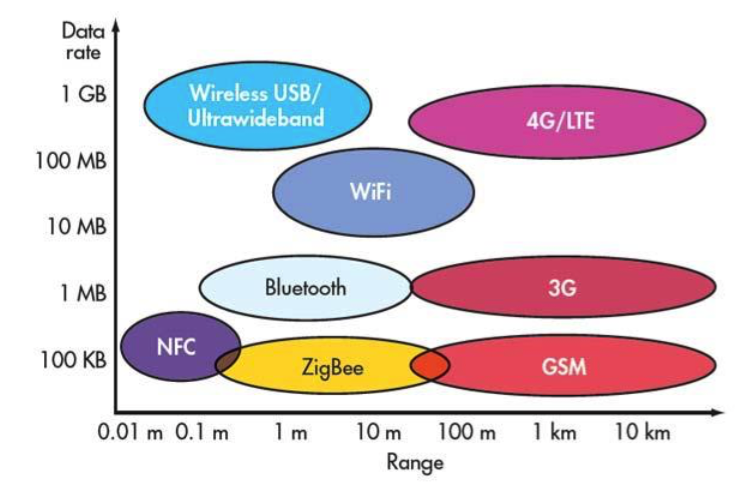
\includegraphics[width=5.00521in,height=3.05208in]{image10.png}
  \end{quote}
\end{itemize}

\subsection{Divisione dello spettro elettromagnetico}
Lo spettro elettromagnetico è diviso in bande che possono essere riservate o 
meno, le bande a 2,4GHz e 5GHz sono libere (e utiliozzate da Bluetooth e per 
esempio dal Wi-Fi, che usa 802.11x). In generale più bassa è la frequenza più il 
segnale è in grado di coprire distanze maggiori ma è in grado di raggiungere 
data-rate meno elevati, più la frequenza è alta invece, maggiore è la capacità 
di trasportare le informazioni ma le distanze coperte sono minori. Ciò è dovuuto 
al fatto che maggiore la frequenza è, più l'onda interagisce con la materia.

\subsection{802.11 Wireless Local Area
Network}\label{wireless-local-area-network}

802.X è una famiglia di standard per le reti locali e metropolitane, in
particolare 802.11 definisce il \textbf{MAC (Medium Access Control)} e
il \textbf{PHY (Physical layer)} per le reti wireless.

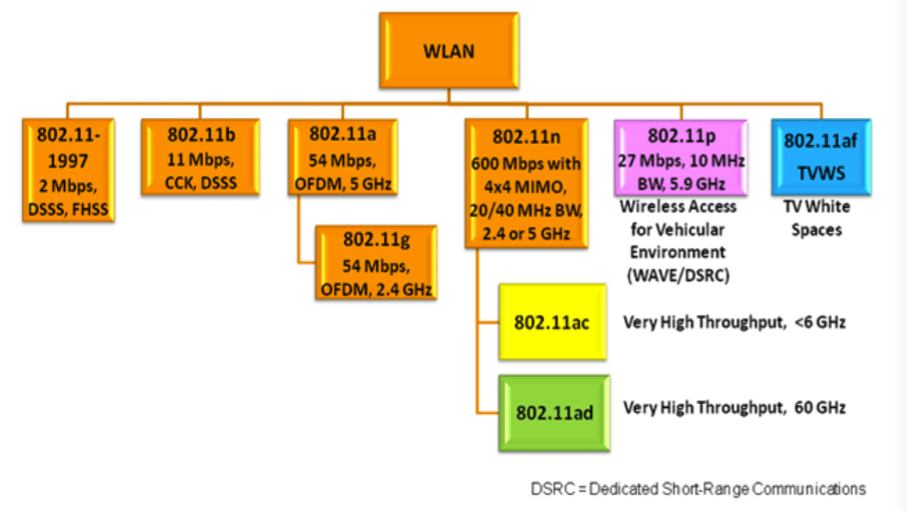
\includegraphics[width=6.26772in,height=3.52778in]{image8.png}

L'obiettivo prefissato per 802.11 è quello di permettere di connettersi
a reti wireless secondo uno standard unico per tutto il mondo, che non
richiede licenze, facile da usare, robusto e che consuma poco. Anche la sicurezza
e la privacy devono essere garantite.

Viene quindi definita una pila di protocolli che specifica come avviene
la comunicazione tra i vari
dispositivi.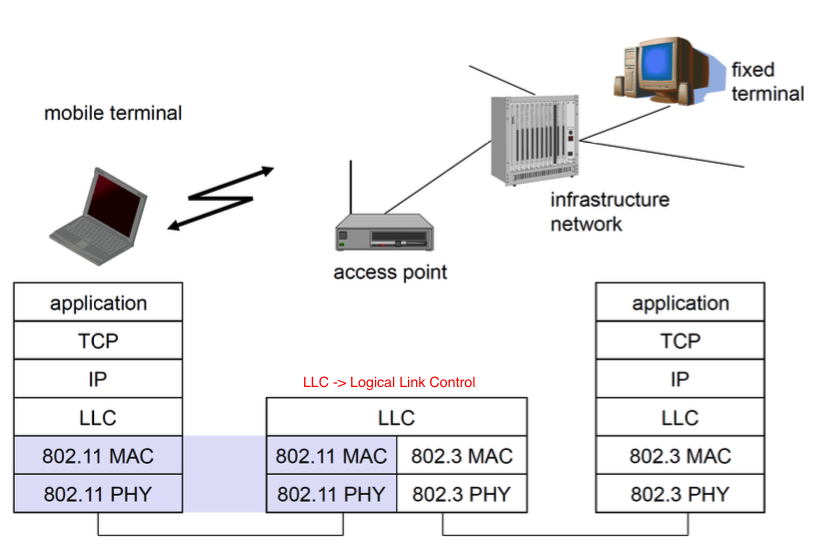
\includegraphics[width=5.29395in,height=3.53844in]{image6a.png}

L'utilizzo tipico prevede un dispositivo mobile che si connette ad un
access point mediante 802.11, l'accesso point è inoltre connesso
all'infrastruttura cablata tramite 802.3, il che permette al dispositivo
mobile di comunicare con tutti i dispositivi connessi alla rete cablata.

Più nel dettaglio, gli strati del MAC e PHY layer sono divisi in vari
componenti:

\begin{itemize}
\item
  \begin{quote}
  \textbf{MAC:} si occupa del meccanismo di accesso al canale, della
  frammentazione dei pacchetti e dell'encryption dei dati.
  \end{quote}
\item
  \begin{quote}
  \textbf{MAC Management}: contiene la logica di sincronizzazione e
  autenticazione
  \end{quote}
\item
  \begin{quote}
  \textbf{PLCP Physical Layer Convergence Protocol:} controlla il canale
  di comunicazione
  \end{quote}
\item
  \begin{quote}
  \textbf{PMD Physical Medium Dependent}: si occupa della codifica e
  modulazione del segnale.
  \end{quote}
\item
  \begin{quote}
  \textbf{Station Management}: si occupa di tutte le funzionalità legate
  alla gestione della stazione di trasmissione.
  \end{quote}
\end{itemize}

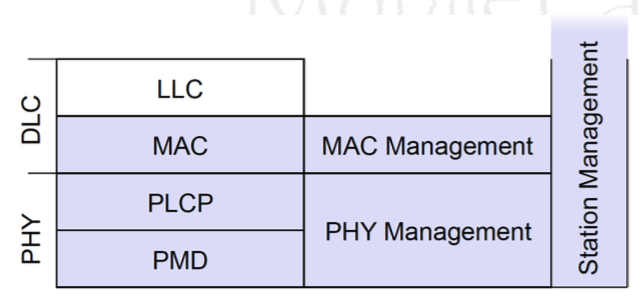
\includegraphics[width=3.98438in,height=1.83334in]{image12.png}

L'accesso al canale può avvenire sfruttando \textbf{CSMA/CA: Carrier Sense
Multiple Access with Collision Avoidance}, ovvero prima di effettuare
una trasmissione viene controllato il canale e viene effettuata una
trasmissione solo se questo è libero. Questo perché non è possibile
effettuare Collision detection. Prima che la trasmissione avvenga viene aspettato
un certo tempo fisso aumentato da un tempo di backoff, aumentato ad ogni 
collisione o ogni volta che il canale risulta occupato (le collisioni possono 
avvenire lo stesso, principalmente perchè il tempo di trasmissione sul canale 
non è nullo).

Ci sono varie versioni dello standard 802.11, ognuna delle quali definisce 
particolari velocità di trasmissioni, frequenze(2,4GHz, 5GHz o entrambi) e 
caratteristiche del dispositivo di trasmissione/modulazione del segnale.

Per gestire la convivenza di più reti wireless è stato predisposto un
meccanismo di canali che utilizzano frequenze di trasmissioni diverse.

\subsubsection{Infrastruttura Vs Ad-Hoc network Vs Wi-Fi
Direct}\label{infrastruttura-vs-ad-hoc-network-vs-wi-fi-direct}

\paragraph{Infrastruttura }\label{infrastruttura}

Tipicamente 802.11 viene utilizzato in modalità \textbf{Infrastruttura},
ovvero ci sono degli access point che collegano una rete wireless ad una
rete cablata, in modo che i dispositivi mobile possono usufruire degli
stessi servizi.

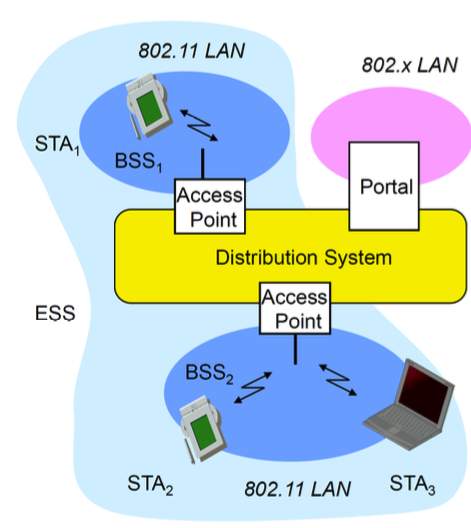
\includegraphics[width=2.88308in,height=3.23438in]{image7.png}

In questo caso si hanno delle \textbf{Station (STA)} che sono dei
terminali con accesso alla rete wireless e che sono in grado di
comunicare con l'access point. Vengono poi identificati vari \textbf{BSS
(Basic Service Set)} che definiscono un gruppo di stazioni che
comunicano sulla stessa frequenza radio. Un \textbf{Access Point} è una
particolare stazione che è connessa sia alla rete wireless che al
sistema di distribuzione dell'infrastruttura (tipicamente la rete
cablata). Un \textbf{Portal} è un ponte che permette la comunicazione
tra due reti diverse (da notare che non è tra AP ad AP), come tra la
rete wireless e quella wired. Il \textbf{Distribution System} è un
interconnessione di reti eterogenee definite da vari \textbf{BSS} che
formano un'unica rete logica che prende il nome di \textbf{Extended
Service Set (ESS)}.

Il set-up della rete wireless viene gestito da un amministratore, il
quale stabilisce i canali di trasmissione dei vari access point, stando
attendo a limitare le interferenze. I vari host si connetteranno poi a
uno degli access point secondo il seguente procedimento:

\begin{enumerate}
\def\labelenumi{\arabic{enumi}.}
\item
  \begin{quote}
  Ascoltano il canale per cercare dei \textbf{beacon frame} che
  descrivono l'access point (nome \textbf{SSID} e MAC address).
  \end{quote}
\item
  \begin{quote}
  Selezionano l'access point a cui associarsi.
  \end{quote}
\item
  \begin{quote}
  Effettuano l'autenticazione (opzionale)
  \end{quote}
\item
  \begin{quote}
  Ottengono un IP, tipicamente assegnato in DHCP, valido per la
  sotto-rete definita dall'access point.
  \end{quote}
\end{enumerate}

Una volta associato o connesso, l'host comunicherà con tutti gli altri
host collegati in rete mediante l'access point (no connesione diretta).

\paragraph{Ad Hoc}\label{ad-hoc}

Nella modalità \textbf{Ad-Hoc} la comunicazione è invece limitata
all'interno di un singolo \textbf{BSS}, che in questo caso prende il
nome di \textbf{Independent Basic Service Set}, in quanto non è
collegato con un sistema di distribuzione.

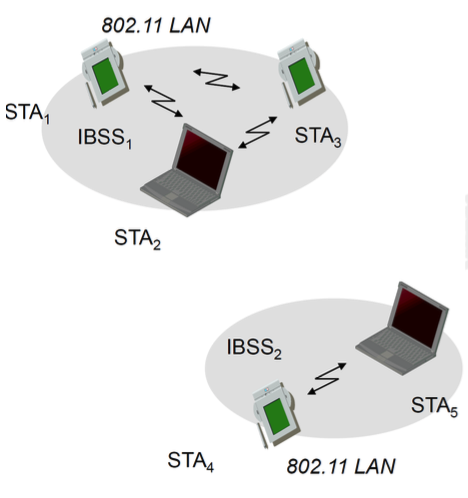
\includegraphics[width=3.11785in,height=3.31771in]{image11.png}

In questo caso il meccanismo di creazione della rete e associazione è
diverso. In primo luogo è necessario un dispositivo che sia in grado di
avviare un \textbf{IBSS} che inizia a trasmettere un beacon con SSID,
BSSID e TSF (timer value). Gli altri dispositivi si connettono alla rete
così creata e a turno si prendono l'onere di trasmettere il beacon
identificativo. In questo caso non ci sono obblighi legati alla
sicurezza/crittografia/autenticazione.

\paragraph{WiFi-Direct o P2P}\label{wifi-direct-o-p2p}

Standard a livello applicazione che permette a due dispositivi di connettersi 
tra loro senza infrastruttura. Questo avviene perché un dispositivo agisce come 
soft access point (AP) o \textbf{group-owner} (\textbf{GO}), mentre gli altri si 
connettono come se fossero delle normali stazioni. Tali ruoli sono decisi nelle 
fasi preliminari di connessione e possono cambiare nel tempo a seguito di una 
ri-negoziazione. Lo standard non vieta la possibilità di creare multigruppi.

La scoperta di un gruppo da parte di una stazione avviene inviando un messaggio 
sonda (probe) per individuare dei GO(di conseguenza dei gruppi) o altri 
dispositivi che non appartengono ad alcun gruppo, nel quale vengono specificate 
le caratteristiche del dispositivo. La risposta a questo messaggio, nel caso 
arrivi da un GO, contiene le caratteristiche del gruppo stesso. Nel caso si 
voglia formare un nuovo gruppo viene prima di tutto definito il dispositivo
che avrà il ruolo di GO. Fatto ciò, viene effettuata una fase di 
\textbf{WPS (WiFi Proteced Set Up)}, ed infine stabiliti gli IP, mediante DHCP. 
Nel caso il gruppo sia già formato, invece, la parte di negoziazione viene 
saltata. L'SSID delle reti WiFi-Direct è della forma `DIRECT-randomNumber'.
Una volta formato il gruppo, GO e clients possono andare in modalità risparmio energetico 
periodicamente, nei periodi di inattività.

Il supporto per i dispositivi mobile però è abbastanza limitato, a differenza per 
esempio di TV o stampanti. Per ovviare a tale problema ci sono soluzioni a 
livello applicazione (o è possibile utilizzare dispositivi con il root, nel caso 
di Android).

La differenza principale tra reti Wi-Fi Direct e MANETs è che nelle prime 
viene deciso un dispositivo che farà da access point e di conseguenza tutte le 
comunicazioni della rete dovranno fluire attraverso tale dispositivo. Nelle reti
Ad-hoc invece è possibile implementare effettivamente il P2P, poichè ogni 
dispositivo è in grado di indirizzare i propri messaggi verso tutte le altre 
stazioni della rete.

I vantaggi delle MANET rispetto al Wi-Fi Direct sono la scalabilità e la 
capacità di gestire cambi di topologia dinamici, unito al fatto che il 
protocollo per reti ad-hoc è molto semplice. Dall'altro canto però nelle MANET 
non è prevista alcuna funzionalità di sicurezza o crittografia automatica, 
previsti invece dal Wi-Fi Direct, ed inoltre la "scoperta" di altri dispositivi
non viene fatta in automatico (in Wi-Fi Direct è prevista dal protocollo).

\subsection{802.15 Personal Area Network}\label{personal-area-network}

L'obiettivo di questo standard è di definire una rete wireless a corto
raggio e con consumi ridotti.

\paragraph{Bluetooth - IEEE 802.15.1}
L'idea fondamentale di \textbf{Bluetooth} è di fornire un'interfaccia comune per 
le comunicazioni wireless ad-hoc, mantenendo:
\begin{itemize}
  \item costi bassi;
  \item raggio d'azione piuttosto corto: il range è 1-100m ma tipicamente non si 
        va oltre i 10m;
  \item limitando il consumo energetico: infatti Bluetooth consuma meno sia del 
        3G che del Wi-Fi. 
\end{itemize}
Cercando di mantenere una velocità di trasmissione accettabile (2.1Mbps).
Tale tecnologia sfrutta la banda a 2.4GHz che, però, essendo libera, è 
utilizzata da molte altre tecnologie. 

Bluetooth utilizza 2 tipologie di accesso al canale: 
\begin {itemize}
  \item \textbf{FHSS(Frequency Hopping Spread Spectrum) con TDD(Time Division 
        Duplex)}, cioè la frequenza di comunicazione viene cambiata in un modo 
        pseudo-random noto sia al trasmettitore che al ricevente, simulando che 
        il canale di comunicazione sia full duplex anche se è half duplex (viene 
        simulato un canale che può essere utilizzato per l'invio e la ricezione 
        simultanea con un canale che permette solo una di queste due alla volta);
  \item \textbf{AFH(Adaptive Frequency Hopping)}, una variante del FHSS nella 
        quale si cerca di evitare di utilizzare dei canali che sono già in uso 
        da altri dispositivi.
\end{itemize}

Un dispositivo che utilizza Bluetooth può essere in uno dei seguenti stati:
\begin{itemize}
  \item Stand-by: quando è disconnesso dalla rete;
  \item Inquiry: quando sta cercando altri dispositivi Bluetooth;
  \item Page: quando è connesso ad un altro dispositivo;
  \item Connected: quando è parte di una piconet;
  \item Parked: quando è addormentato per risparmiare più energia possibile;
  \item Sniff: quando controlla il canale periodicamente al posto di essere 
        sempre in ascolto (risparmio energetico)
  \item Hold: quando si addormenta per un determinato periodo, passato il quale 
        ritorna in uno stato attivo.
\end{itemize}

Questa tecnologia prevede che un certo dispositivo implementi uno o più profili, 
ovvero una serie di protocolli che definiscono lo scopo per il quale Bluetooth è 
sfruttato (esempi di profili sono: trasmissione di file, telefonia cordless, 
accesso rete LAN, sincronizzazione, ...).

Tramite il bluetooth i dispositivi creano delle reti a stella chiamate 
\textbf{piconet}. In ogni piconet è presente un master e al massimo 7 slave 
attivi (ce ne possono essere più di 200 in stato non attivi)

Più piconet possono essere unite per formare una \textbf{scatternet}: in questo 
caso la congiunzione tra le due reti avviene tramite uno dei dispositivi, con la 
limitazione che questo non può essere master in entrambe le reti che unisce(può 
essere master in una e slave nell'altra o slave in entrambe).

\paragraph{BLE - Bluetooth Low Energy}
BLE è un'evoluzione del classico Bluetooth, rilasciata nel 2010, che ne migliora 
le performance. Infatti BLE, oltre ad essere più veloce, consuma meno energia ed 
è meno costoso. Ciò deriva dal fatto che il chip responsabile delle trasmissioni 
è inattivo per la maggior parte del tempo ed è stata diminuita la dimensione 
massima dei pacchetti scambiati. Oltre a ciò BLE aggiunge nuovi profili.

\paragraph{IEEE 802.15.4}
Lo IEEE 802.15.4 è uno standard per le comunicazione nelle PAN a bassissimi:
\begin{itemize}
  \item costo;
  \item velocità;
  \item energia.
\end{itemize}

I dispositivi che lo sfruttano sono pensati per avere una batteria che dura 
molto a lungo (anche un paio d'anni), di facile utilizzo e basso costo. Tale 
standand è utilizzato per esempio nei giocattoli interattivi e per reti 
domestiche.

La banda utilizzata è sempre quella a 2,4GHz, poichè libera, al quale viene 
aggiunta una banda a 868MHz, in Europa, e a 915MHz, negli USA.

I dispositivi che sfruttano lo IEEE 802.15.4 possono essere divisi in 
\textbf{full function device (FFD)}, i quali implementano tutte le funzionalità 
previste dal protocollo, \textbf{reduced function device (RFD)}, che invece ne 
prevedono solamente un sottoinsieme e possono essere solamente impiegati come 
foglie nelle reti, e \textbf{PAN coordinator}, che hanno lo scopo di fare da 
coordinatori alla rete.

Nelle reti con topologia a stella ci sarà un PAN coordinator come noddo centrale 
e una combianazione qualsiasi delle altr due tipologie come foglie della rete. 
Nelle reti ad albero, invece, il PAN coordinator sarà la radice dell'albero, gli 
RFD le foglie, mentre gli FFD potranno essere sia foglie che nodi interni. 

%=========MANCA P2P PER 802.15.4 pg 55 e poi da pg 57===================================